\chapter{Mixed-Bag Solver Overview}

This thesis' Mixed-Bag Solver supports Type~1, Type~2, and Mixed-Bag Puzzles.  It consists of five distinct stages namely: segmentation, stitching piece solving, hierarchical clustering of segments, seed piece selection, and final assembly.  The flow of the algorithm is shown in Figure~\ref{fig:multipuzzleSolverArchitecture}.

The following subsections describe each of the components solver architecture.  It also discusses the assembler which is an independent but associated component of the architecture.

\begin{figure}[ht!]
	\centering
		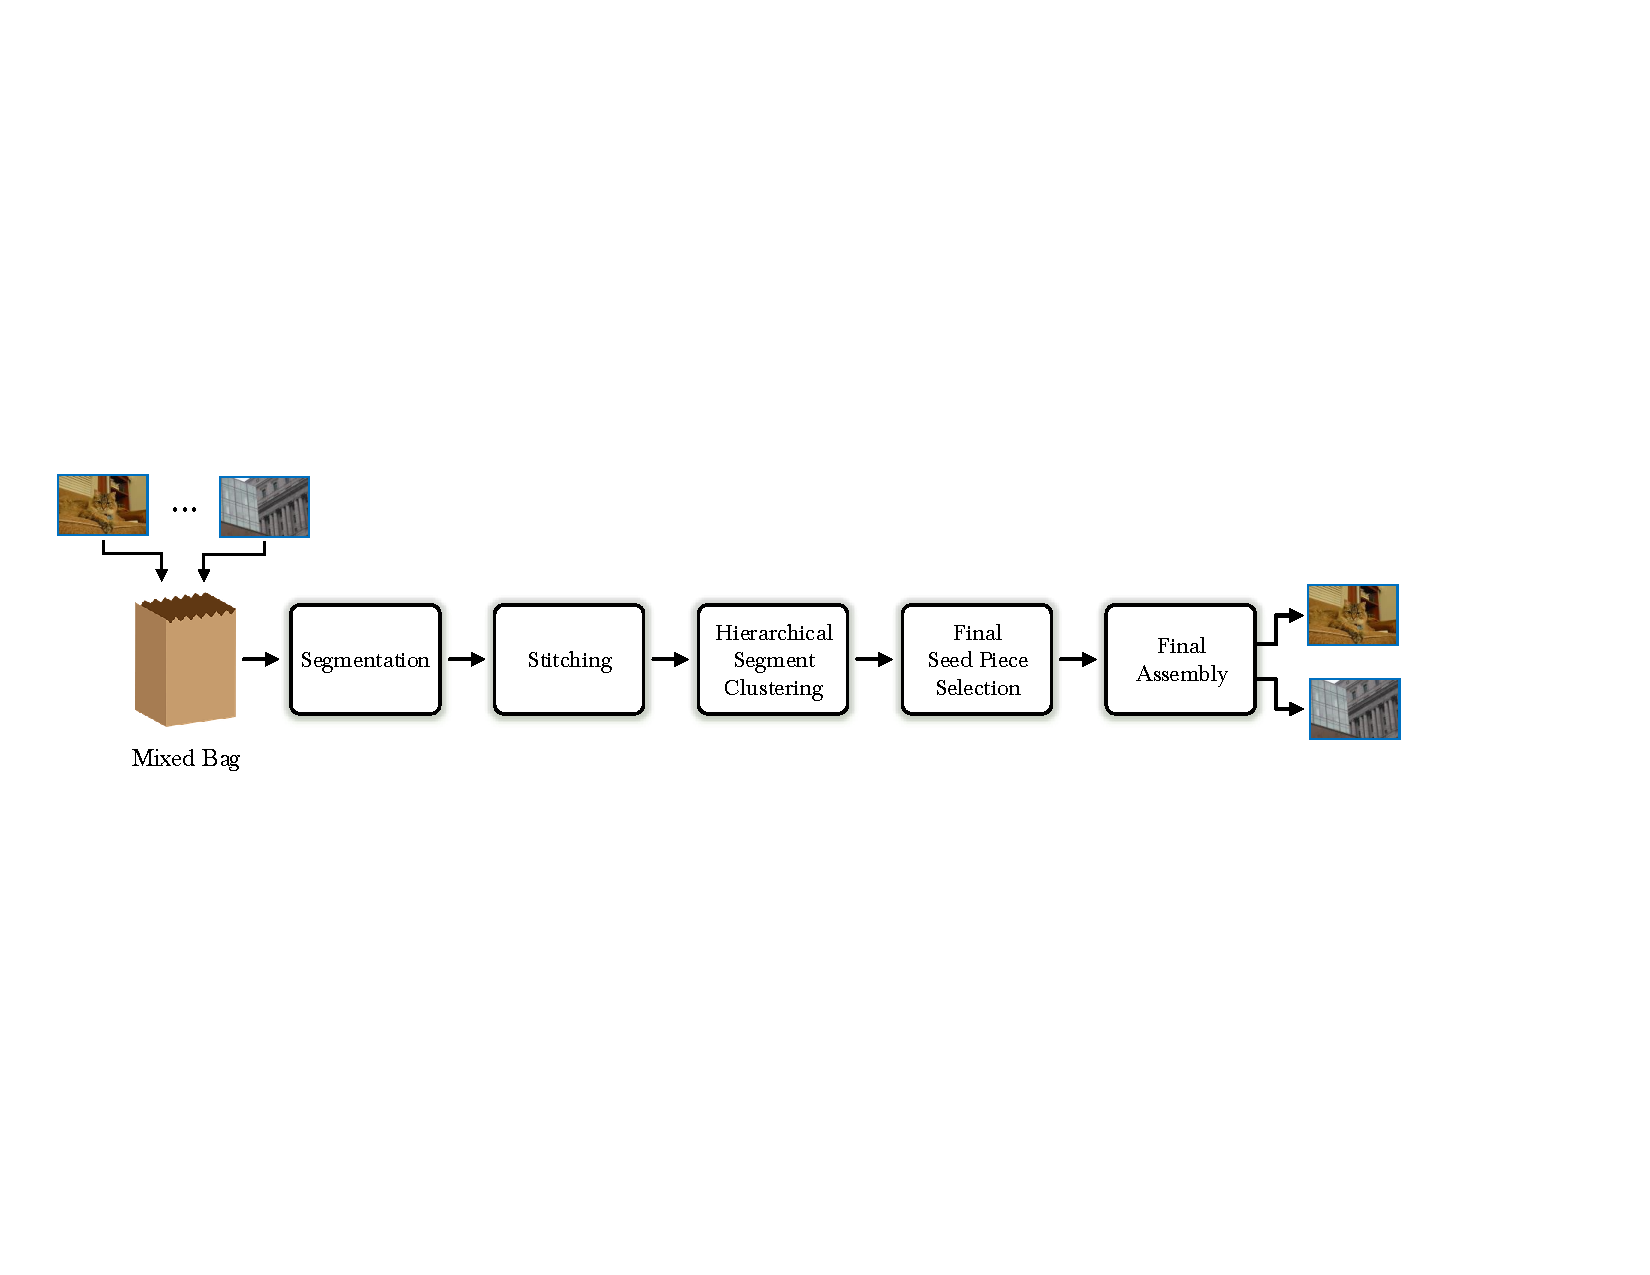
\includegraphics[width=1.0\textwidth]{images/cropped_algorithm_structure_overview.pdf}
	\caption{Components of the Mixed-Bag Puzzle Solver}\label{fig:multipuzzleSolverArchitecture}
\end{figure}

\section{Assembler}\label{sec:SolverAssembler}

The role of the assembler assigns the placement (and optionally rotation) of the puzzle pieces in the solved puzzle.  This solver architecture is largely independent of the assembler used.  Hence, as assemblers improve, they can be incorporated into this solver to improve the overall performance.  The same also applies if particular assembler(s) perform better for particular types of puzzles.  This enables significant flexibility to balance competing concerns, while maintaining upgradability.

For all experiments in this thesis, we used the solver proposed by Paikin \& Tal \cite{paikin2015}.  It was selected because it the current state-of-the-art.  What is more, since it supports mixed bag puzzles, it can be used for direct comparison of performance.

\section{Segmentation}\label{sec:Segmentation}

The first stage in the Mixed-Bag Solver is the Segmentation.  It takes as input only the bag of puzzle pieces created from the original images; unlike all other solvers to date, this algorithm takes no other inputs.  The role of segmentation is to provide structure to the unordered input by partitioning the pieces into disjoint sets, referred to here as segments.  This is done by determining segments of the puzzle that solved correctly and retaining them further further analysis.  The following subsections discuss the segmentation procedure.

\subsection{The Segmentation Procedure}


As mentioned previously, all of the puzzle pieces supplied to the algorithm are passed into the segmentation procedure (see Algorithm~\ref{alg:segmentation}).  The solver then assembles the puzzle(s) as if all pieces came from a single ground truth image.  This eliminates the need for the algorithm to estimate the number of input puzzles until very late in the solving process.  It is possible that this approach may cause some areas of the puzzle to be assembled poorly. 


\begin{algorithm}
\caption{Segmentation}\label{alg:segmentation}
\begin{algorithmic}[1]
\Procedure{Segmentation}{$all\_pieces$}
    \State $\textit{saved\_segments} \gets \{ \}$
    \State $\textit{unassigned\_pieces} \gets \{ \textit{all\_pieces} \}$
    \Do
        \State $\textit{solved\_puzzle} \gets \textbf{run\_single\_assembly}(\textit{unassigned\_pieces})$
        \State $\textit{solved\_segments} \gets \textbf{segment\_puzzle}(\textit{solved\_puzzle})$
        \State $\textit{max\_segment\_size} \gets \text{maximum size of segment in } \textit{solved\_segments}$
        \ForAll{$\textit{segment} \in \textit{solved\_segments}$}
            \If{$|\textit{segment}| \text{>} \alpha \times \textit{max\_segment\_size}$}
                \State $\text{add } \textit{segment} \text{ to } \textit{saved\_segments}$
                \State $\text{remove pieces in } \textit{segment} \text{ from } \textit{unplaced\_pieces}$
            \EndIf
        \EndFor
    \doWhile{$\textit{max\_segment\_size} \text{>} \textit{smallest\_allowed} \textbf{ and } |\textit{unplaced\_pieces}| \text{>} 0$}
\EndProcedure
\end{algorithmic}
\end{algorithm}

After the solver is run in each segmentation round, the output is divided into disjoint sets or segments by the method "\texttt{segment\_puzzle};'' its procedure is described in Section~\ref{sec:segmentPuzzle}.

The largest segment in each round i

For a segment to be saved for future analysis, it must be larger than a predefined minimum size.  In this thesis' implementation, a minimum segment size of 7 provided the best balance between execution time and segment granularity.

\subsubsection{{segment\_puzzle} Procedure}\label{sec:segmentPuzzle}

The \texttt{segment\_puzzle} procedure shown in Algorithm~\ref{alg:segmentPuzzle} is adapted from the kernel growing segmentation procedure modified by Pomeranz \textit{et al.}, where it was shown to have greater than 99.7\% accuracy identifying genuine neighbors \cite{pomeranz2011}. The kernel of each segment is a single seed piece.

\begin{algorithm}
\caption{Segment Puzzle}\label{alg:segmentPuzzle}
\begin{algorithmic}[1]
\Procedure{segment\_puzzle}{$solved\_puzzle$}
    \State $\textit{solved\_segments} \gets \{ \}$
    \State $\textit{unassigned\_pieces} \gets \{ \text{all pieces in } \textit{solved\_puzzle} \}$
\item[]
    \While{$|\textit{unassigned\_pieces}| \text{>} 0$}
        \State $\textit{segment} \gets \text{ new empty segment}$
        \State $\textit{seed\_piece} \gets \text{next piece in } \textit{unassigned\_pieces}$
        \State $\textit{queue} \gets [\textit{seed\_piece}]$
\item[]
        \While{$|\textit{queue}| \text{>} 0$}
            \State $\textit{piece} \gets \text{next piece in }\textit{queue}$
            \State $\text{add } \textit{piece} \text{ to } \textit{segment}$
\item[]
            \ForAll{$\textit{neighbor\_piece} \text{ of } \textit{piece}$}
            	\If{$\textbf{is\_best\_buddies}(\textit{neighbor\_piece}, \textit{piece})$}
            		\State $\text{add } \textit{neighbor\_piece} \text{ to } \textit{queue}$
            		\State $\text{remove } \textit{neighbor\_piece} \text{ from } \textit{unassigned\_pieces}$
            	\EndIf
            \EndFor
        \EndWhile
\item[]
        \State $\textit{articulation\_points} \gets \textbf{find\_articulation\_points}(\textit{segment})$
        \State $\text{remove } \textit{articulation\_points} \text{ from } \textit{segment}$
\item[]
		\State $\textit{disconnected\_points} \gets \textbf{get\_disconnected\_points}(\textit{segment},\textit{seed\_piece})$        
        \State $\text{remove } \textit{disconnected\_points} \text{ from } \textit{segment}$
\item[]
        \State $\text{add } \textit{articulation\_points} \text{ and } \textit{disconnected\_points} \text{ to } \textit{unassigned\_pieces}$
    \EndWhile
\EndProcedure
\end{algorithmic}
\end{algorithm}

Whenever a piece is added to a segment, it is removed from the set of unassigned pieces. What is more, the algorithm check's all pieces directly adjacent to the added piece.  If the adjacent piece and the added piece are "best buddies'' (i.e., each is more similar to the other on their respective sides than they are to any other piece as defined by \cite{pomeranz2011} and \cite{paikin2015}), then the adjacent piece is also added to the segment.  This process continues until no there are no pieces adjacent to a segment member that fulfill the best buddy criteria.

If Pomeranz \textit{et al.}'s original segmentation algorithm is used for Mixed-Bag puzzles, two correctly assembled segments from different input puzzles can be merged into a single segment.  This is usually in the form of narrow bridges no wider than a single piece. This necessitates that each segment goes through post-processing to identify and remove these single point bridges; the procedure for doing this is described in Section~\ref{sec:ArticulationPoints}.  

Once these single piece bridges have been broken, one or more pieces become disconnected from the segment.  These pieces are then returned to the set of unassigned pieces to be assigned to a different segment.  At the end of segment, each piece in the puzzle will be assigned to exactly one segment.

\subsubsection{Articulation Points}\label{sec:segmentPuzzle}

A segment can be model as a single connected graph, with the vertices being the puzzle pieces and the edges being the best buddy relationships.  An articulation point is any vertex (\textit{i.e.}, puzzle piece) whose removal increases the number of connected components.  The Mixed-Bag Solver uses the algorithm proposed by \ref{cormen} for identifying articulation points.  While most implementations of this algorithm are recursive, this thesis instead uses an iterative approach as segment can be several thousand pieces in sizes.  As such, a recursive implementation is prone to stack overflows.

